\documentclass[12pt]{scrartcl}

\usepackage[T1]{fontenc}
\usepackage[utf8]{inputenc}
\usepackage{amsmath}
\usepackage{amsfonts}
\usepackage{amssymb}
\usepackage{amsbsy}
\usepackage{graphicx}
\usepackage{float}
\usepackage{array}
\usepackage{booktabs}
\usepackage{multirow}
\usepackage{bm}
\usepackage{verbatim}
\usepackage[english]{babel}
\usepackage{color}
\usepackage{url}
\usepackage{fancybox}
\usepackage[stable]{footmisc}
\usepackage[format=plain,labelfont=bf]{caption}
\usepackage{fancyhdr}
\usepackage{natbib}
\usepackage{calc}
\usepackage{textcomp}
\usepackage[pdftex,pdfborder={0 0 0}]{hyperref}
\usepackage{pdfpages}
\usepackage{tikz}
\usetikzlibrary{shapes,backgrounds,fit,positioning,arrows,positioning,decorations.pathmorphing,decorations.pathreplacing,backgrounds}
\usepackage{accents}
\usepackage{placeins}

\renewcommand*{\familydefault}{\sfdefault}

% Margins
\addtolength{\textheight}{1.0cm}
\addtolength{\oddsidemargin}{-0.5cm}
\addtolength{\evensidemargin}{-0.5cm}
\addtolength{\textwidth}{1.0cm}
\parindent=0em

% Appropriate font for \mathcal{}
\DeclareSymbolFont{cmmathcal}{OMS}{cmsy}{m}{n}
\DeclareSymbolFontAlphabet{\mathcal}{cmmathcal}

% Set subscript and superscripts positions
\everymath{
\fontdimen13\textfont2=5pt
\fontdimen14\textfont2=5pt
\fontdimen15\textfont2=5pt
\fontdimen16\textfont2=5pt
\fontdimen17\textfont2=5pt
}

% Bibliography style
\setlength{\bibsep}{1pt}

% Part
\renewcommand\partheadstartvskip{\clearpage\null\vfil}
\renewcommand\partheadmidvskip{\par\nobreak\vskip 20pt\thispagestyle{empty}}
\renewcommand\partheadendvskip{\vfil\clearpage}
\renewcommand\raggedpart{\centering}

\begin{document}
\title{Biperiodization: the SEAM method}
\author{Benjamin Ménétrier}
\date{Last update: \today}

\thispagestyle{empty}

\maketitle

\tableofcontents

\section{Problem definition}

\subsection{In the NWP world}

In Numerical Weather Prediction models, the biperiodization process is needed to make a large scale non-periodic 2D field periodic over a limited-area domain, in order to apply discrete Fourier transforms. For this purpose, the original domain (called the ``physical zone'') is extended on two sides. This artificial "extension zone" has to be filled with adequate values to make the whole field periodic.\\
$  $\\
The work of \cite{blazica_2015} reviews existing methods, and can be quickly summarized as follows:
\begin{itemize}
\item The extension methods of HIRLAM and ALADIN models are based on spline (ALADIN) or trigonometric (HIRLAM) functions, which are applied in both directions successively. They lead to wild overshoots in the extension zone and have a strong impact on the spectra.
\item The detrending approach requires a modification of the physical values.
\item The Boyd method is very good but requires data from outside the physical zone (e.g. from a large scale coupler).
\item The discrete cosine transform method produces accurate spectra but increases the total domain size by a factor 4.
\end{itemize}

In this note, we focus on methods that do not change the physical values (excluding the detrending approach), rely on the values within this physical zone only (excluding the Boyd method), and are computationally efficient (excluding the discrete cosine transform method). Thus, we try to find a better alternative to the extension methods of HIRLAM and ALADIN.

\subsection{In a simplified framework}

Biperiodization methods can be designed and tested in an idealized 1D framework, as a "gap filling" problem. The goal is to define values in a missing segment with several objectives:
\begin{itemize}
\item ensuring the signal continuity, and if possible the continuity of its derivatives,
\item avoiding overshoots, i.e. values significantly out of the range of the original values,
\item keeping the signal scales to avoid spectrum distorsion.
\end{itemize} 

Figure \ref{fig:detail_init} shows a smooth random signal with missing data, which we will use for illustration purposes. The spline method is illustrated in figure \ref{fig:detail_spline}: while the signal continuity is good, an overshoot is clearly visible over the red bar and the signal is smoother in the filled area than outside of it.

\begin{figure}[!ht]
\center
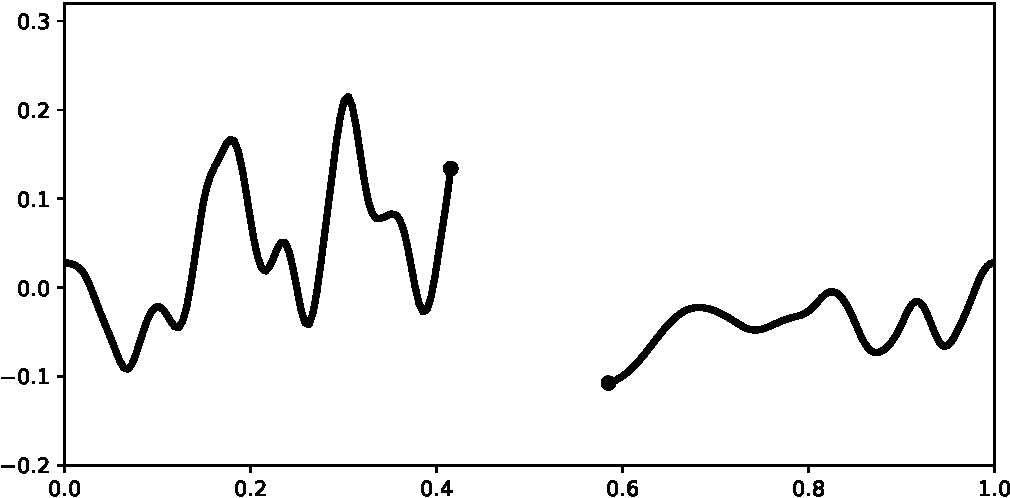
\includegraphics[width=0.7\textwidth]{detail_init.pdf}
\caption{Smooth random signal with missing data}
\label{fig:detail_init}
\end{figure}
\FloatBarrier

\begin{figure}[!ht]
\center
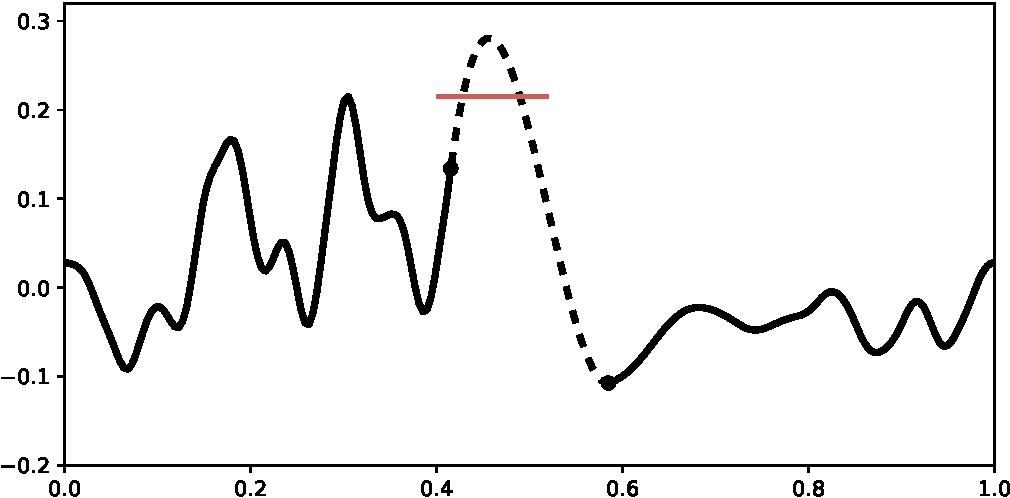
\includegraphics[width=0.7\textwidth]{detail_spline.pdf}
\caption{Gap filled with the spline method (dashed black)}
\label{fig:detail_spline}
\end{figure}
\FloatBarrier

\section{The SEAM method}

The SEAM method stands for ``Symmetric Extension And Mixing'', and will be described in this section.

\subsection{Detailed steps}

In this first step, the signal is extended in the gap based on both symmetric or an antisymmetric extensions from both sides of the gap. Figure \ref{fig:detail_mix_left} extensions starting from the left side of the gap:
\begin{itemize}
\item for the symmetric extension (blue), overshoots are not possible but the signal derivative continuity at the boundary is lost,
\item for the antisymmetric extension (red), overshoots are possible but the signal first two derivatives continuity at the boundary is maintained.
\end{itemize}
Thus, it seems relevant to stay close to the the antisymmetric extension at to the boundary, and then converge to the symmetric extension further away, as shown with the dashed gray curve in Figure \ref{fig:detail_mix_left}. 

\begin{figure}[!ht]
\center
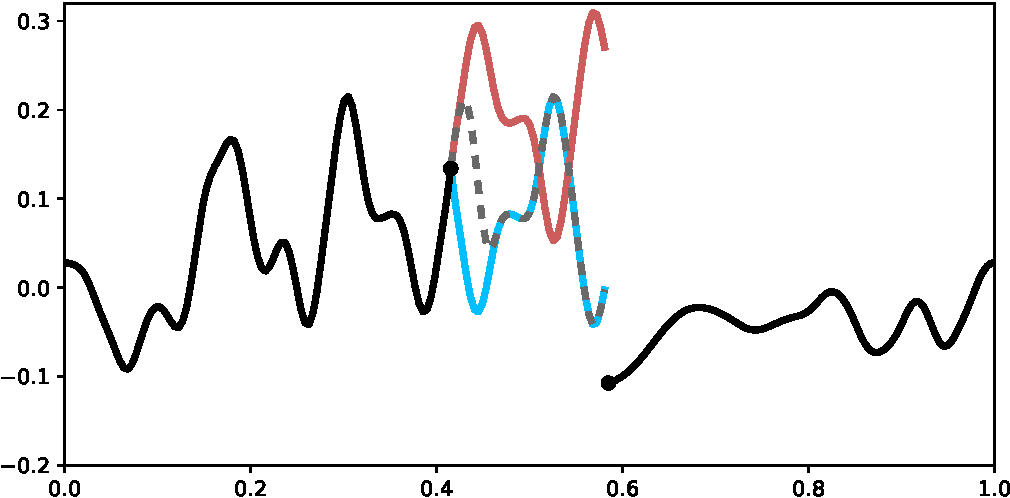
\includegraphics[width=0.7\textwidth]{detail_mix_left.pdf}
\caption{Symmetric (blue), antisymmetric (red) and combined (dahed gray) extensions on the left side of the gap}
\label{fig:detail_mix_left}
\end{figure}
\FloatBarrier

The weights of symmetric and antisymmetric extensions in the linear combination are given by the \cite{boyd_2005} formula. It provides a ramp going from 1 to 0 for an argument going from 0 to 1:
\begin{align}
\mathcal{B}(x) = \frac{1}{2} \left(1+\text{erf}\left(L\frac{1-2x}{\sqrt{4x(1-x)}}\right)\right)
\end{align}

The shape of $\mathcal{B}(x)$ is given in Figure \ref{fig:boyd} for different values of $L$. In this study, we found that the actual value of $L$ is not very sensitive and we keep $L = 1.5$ hereafter.

\begin{figure}[!ht]
\center
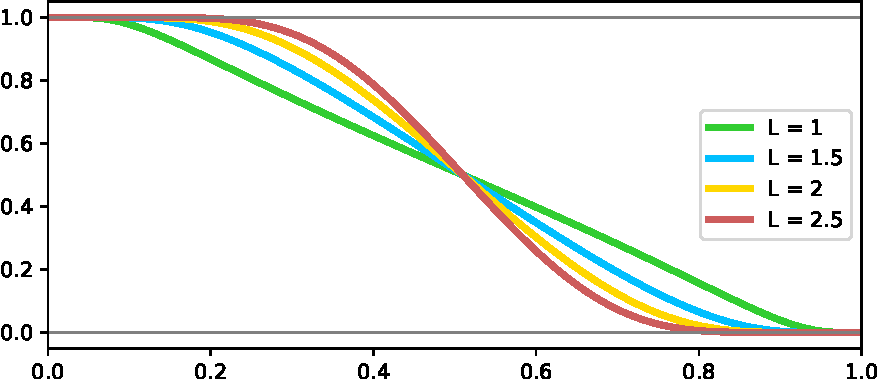
\includegraphics[width=0.7\textwidth]{boyd.pdf}
\caption{Normalized \cite{boyd_2005} ramp functions for various values of the $L$ parameter}
\label{fig:boyd}
\end{figure}
\FloatBarrier

A more critical parameter is the width over which the linear combination is performed, starting from the boundary. Figure \ref{fig:detail_mix_wide_left} shows a case where this combination width is too large, leading to a significant overshoot. So we recommand a rather narrow combination width ($\sim$ 10 points), but large enough to ensure derivatives continuity at the boundary.

\begin{figure}[!ht]
\center
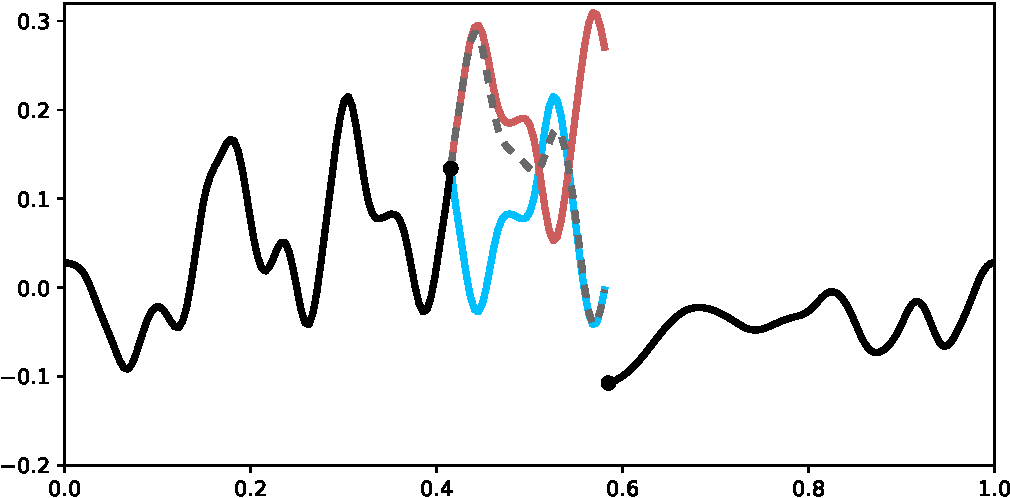
\includegraphics[width=0.7\textwidth]{detail_mix_wide_left.pdf}
\caption{Same as figure \ref{fig:detail_mix_left} with a large combination width}
\label{fig:detail_mix_wide_left}
\end{figure}
\FloatBarrier

The same procedure is applied on the right side of the gap, as shown in Figure \ref{fig:detail_mix_right}.

\begin{figure}[!ht]
\center
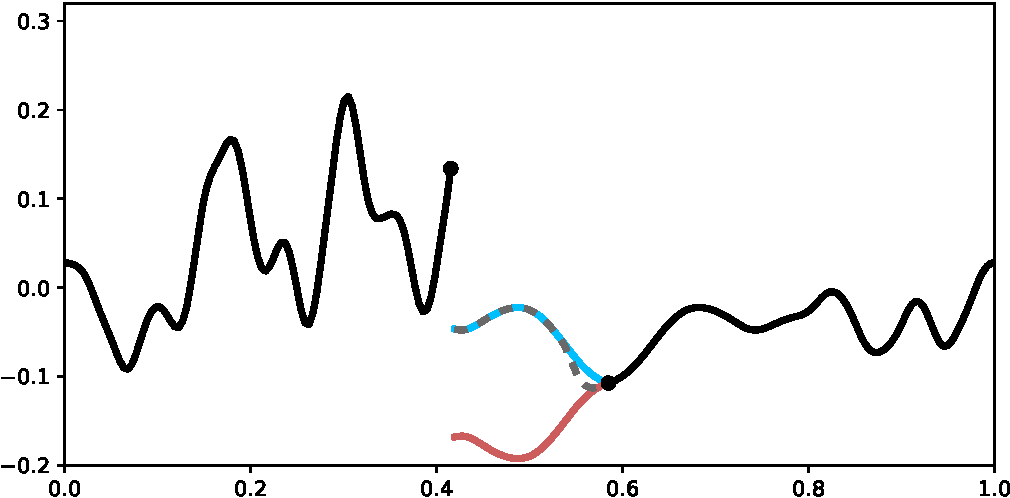
\includegraphics[width=0.7\textwidth]{detail_mix_right.pdf}
\caption{Symmetric (blue), antisymmetric (red) and combined (gray) extensions on the right side of the gap}
\label{fig:detail_mix_right}
\end{figure}
\FloatBarrier

In the final step, we apply the \cite{boyd_2005} method to combine the left side and right side extensions, as shown in Figure \ref{fig:detail_final}.

\begin{figure}[!ht]
\center
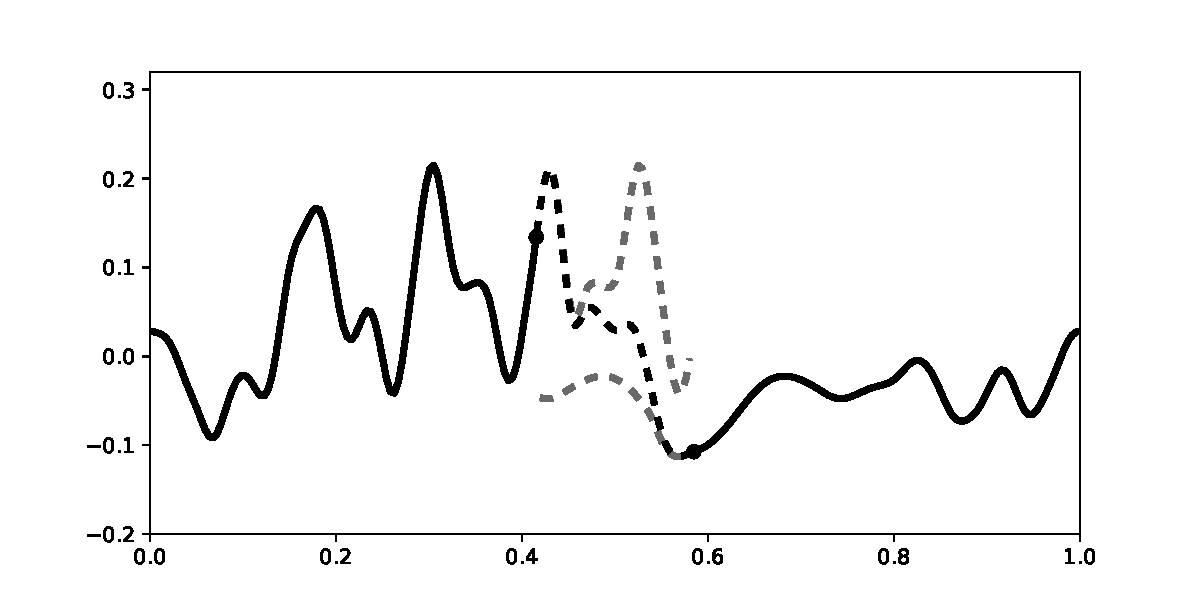
\includegraphics[width=0.7\textwidth]{detail_final.pdf}
\caption{Extensions on both sides of the gap (dashed gray) and final SEAM solution (dashed black)}
\label{fig:detail_final}
\end{figure}
\FloatBarrier

\subsection{2D implementation}

We denote $x$ the input value in the physical zone and $y$ the intermediate and output values in the extension zone. The output value
\begin{align}
y = \sum_{i=1}^n y_i
\end{align}
is the sum of several components $y_1, ..., y_n$ because of the last mixing step in two dimensions, with $n$ depending on the point location in the extension zone:
\begin{itemize}
\item right side: $n=2$
\item top side: $n=2$
\item right-top corner: $n=4$
\end{itemize}

For each component $y_i$, we can define two input points:
\begin{itemize}
\item $x^\text{bnd}_i$: closest points on the physical zone boundary,
\item $x^\text{sym}_i$: symmetric point with respect to $x^\text{bnd}_i$.
\end{itemize}

The symmetric and antisymmetric extensions are respectively given by:
\begin{align}
y^\text{sym}_i & = x^\text{sym}_i \\
y^\text{antisym}_i & = 2 x^\text{bnd}_i - x^\text{sym}_i
\end{align}

For each component, we denote $c^\text{ext}_i$ the local extension combination factor and $c^\text{mix}_i$ the local mixing factor. The final component value is given by:
\begin{align}
y_i = \left(c^\text{ext}_i y^\text{sym}_i + \left(1-c^\text{ext}_i\right) y^\text{antisym}_i \right) c^\text{mix}_i
\end{align}
which can be expressed as a linear combination of input values:
\begin{align}
y_i = \alpha^\text{bnd}_i x^\text{bnd}_i + \alpha^\text{sym}_i x^\text{sym}_i
\end{align}
with the linear coefficients:
\begin{align}
\alpha^\text{bnd}_i & = 2 c^\text{ext}_i c^\text{mix}_i \\
\alpha^\text{sym}_i & = \left(1 - 2 c^\text{ext}_i\right) c^\text{mix}_i
\end{align}

Figure \ref{fig:base_single} shows an exemple of a smooth random 2D field biperiodized with the SEAM method.

\begin{figure}[!ht]
\center
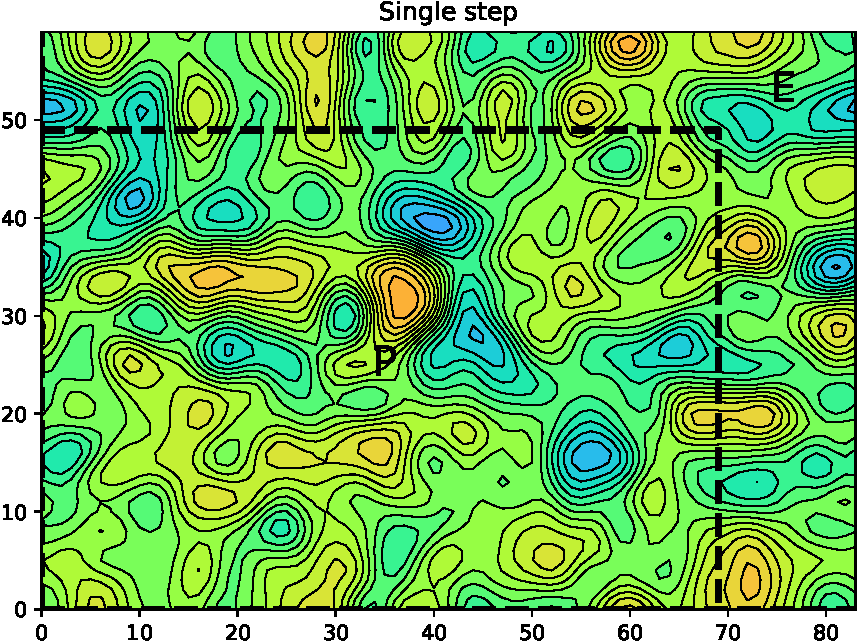
\includegraphics[width=0.7\textwidth]{base_single.pdf}
\caption{Smooth random 2D field biperiodized with the SEAM method, from the physical zone (P) to the extension zone (E)}
\label{fig:base_single}
\end{figure}
\FloatBarrier

\section{Real case tests}

\subsection{Practical implementation in IAL}

In the IAL code, the SEAM method is implemented in \texttt{biper/module/eseam\_mod.F90}. Like the spline or the Boyd methods, it can be called from \texttt{biper/external/fpbipere.F90}. To use the SEAM method from the \texttt{fpbipere} interface, the following optional arguments must be specified:
\begin{itemize}
\item \texttt{ldseam=.true.} to activate the SEAM method
\item \texttt{kdseam} [integer], which contains the combination width
\item \texttt{plseam} [real(2)], which contains the extension combination and mixing lengths for the \cite{boyd_2005} ramp function.
\end{itemize}

\subsection{Methods comparison}
The spline method (with an additional smoothing of overshoots) and the SEAM method have been compared for a low level temperature field. Figure \ref{fig:biperFromIAL} shows that the SEAM method produces a field without overshoots, while keeping the continuity at the boundaries and maintaining the original signal scales. This last property can be confirmed with a variance spectrum computed using the \cite{denis_2002} method. In Figure \ref{fig:biperFromIAL_spectra_80_11}, the SEAM spectrum is closer to the original than the spline spectrum.

\begin{figure}[!ht]
\center
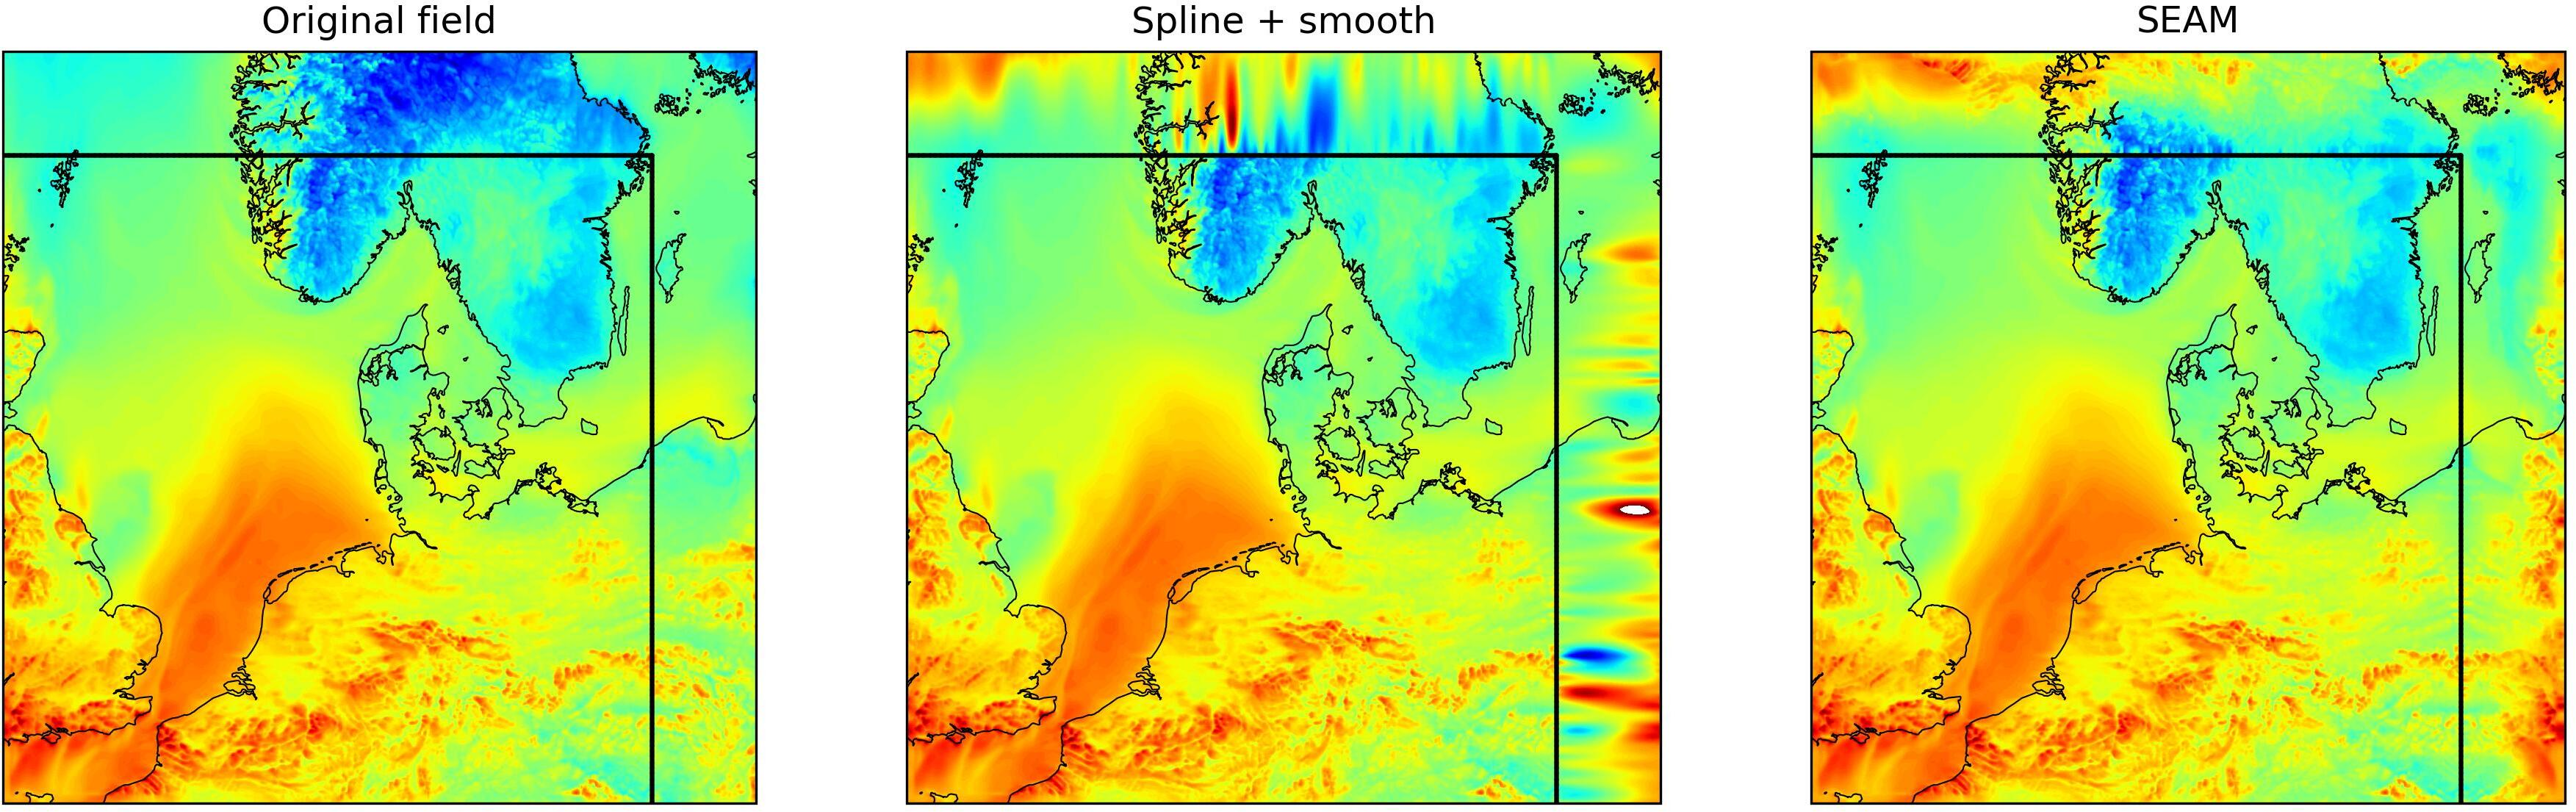
\includegraphics[width=\textwidth]{biperFromIAL.jpg}
\caption{Original non-periodic field (right), biperiodized with the spline+smooth method (center) or the SEAM method (left)}
\label{fig:biperFromIAL}
\end{figure}
\FloatBarrier

\begin{figure}[!ht]
\center
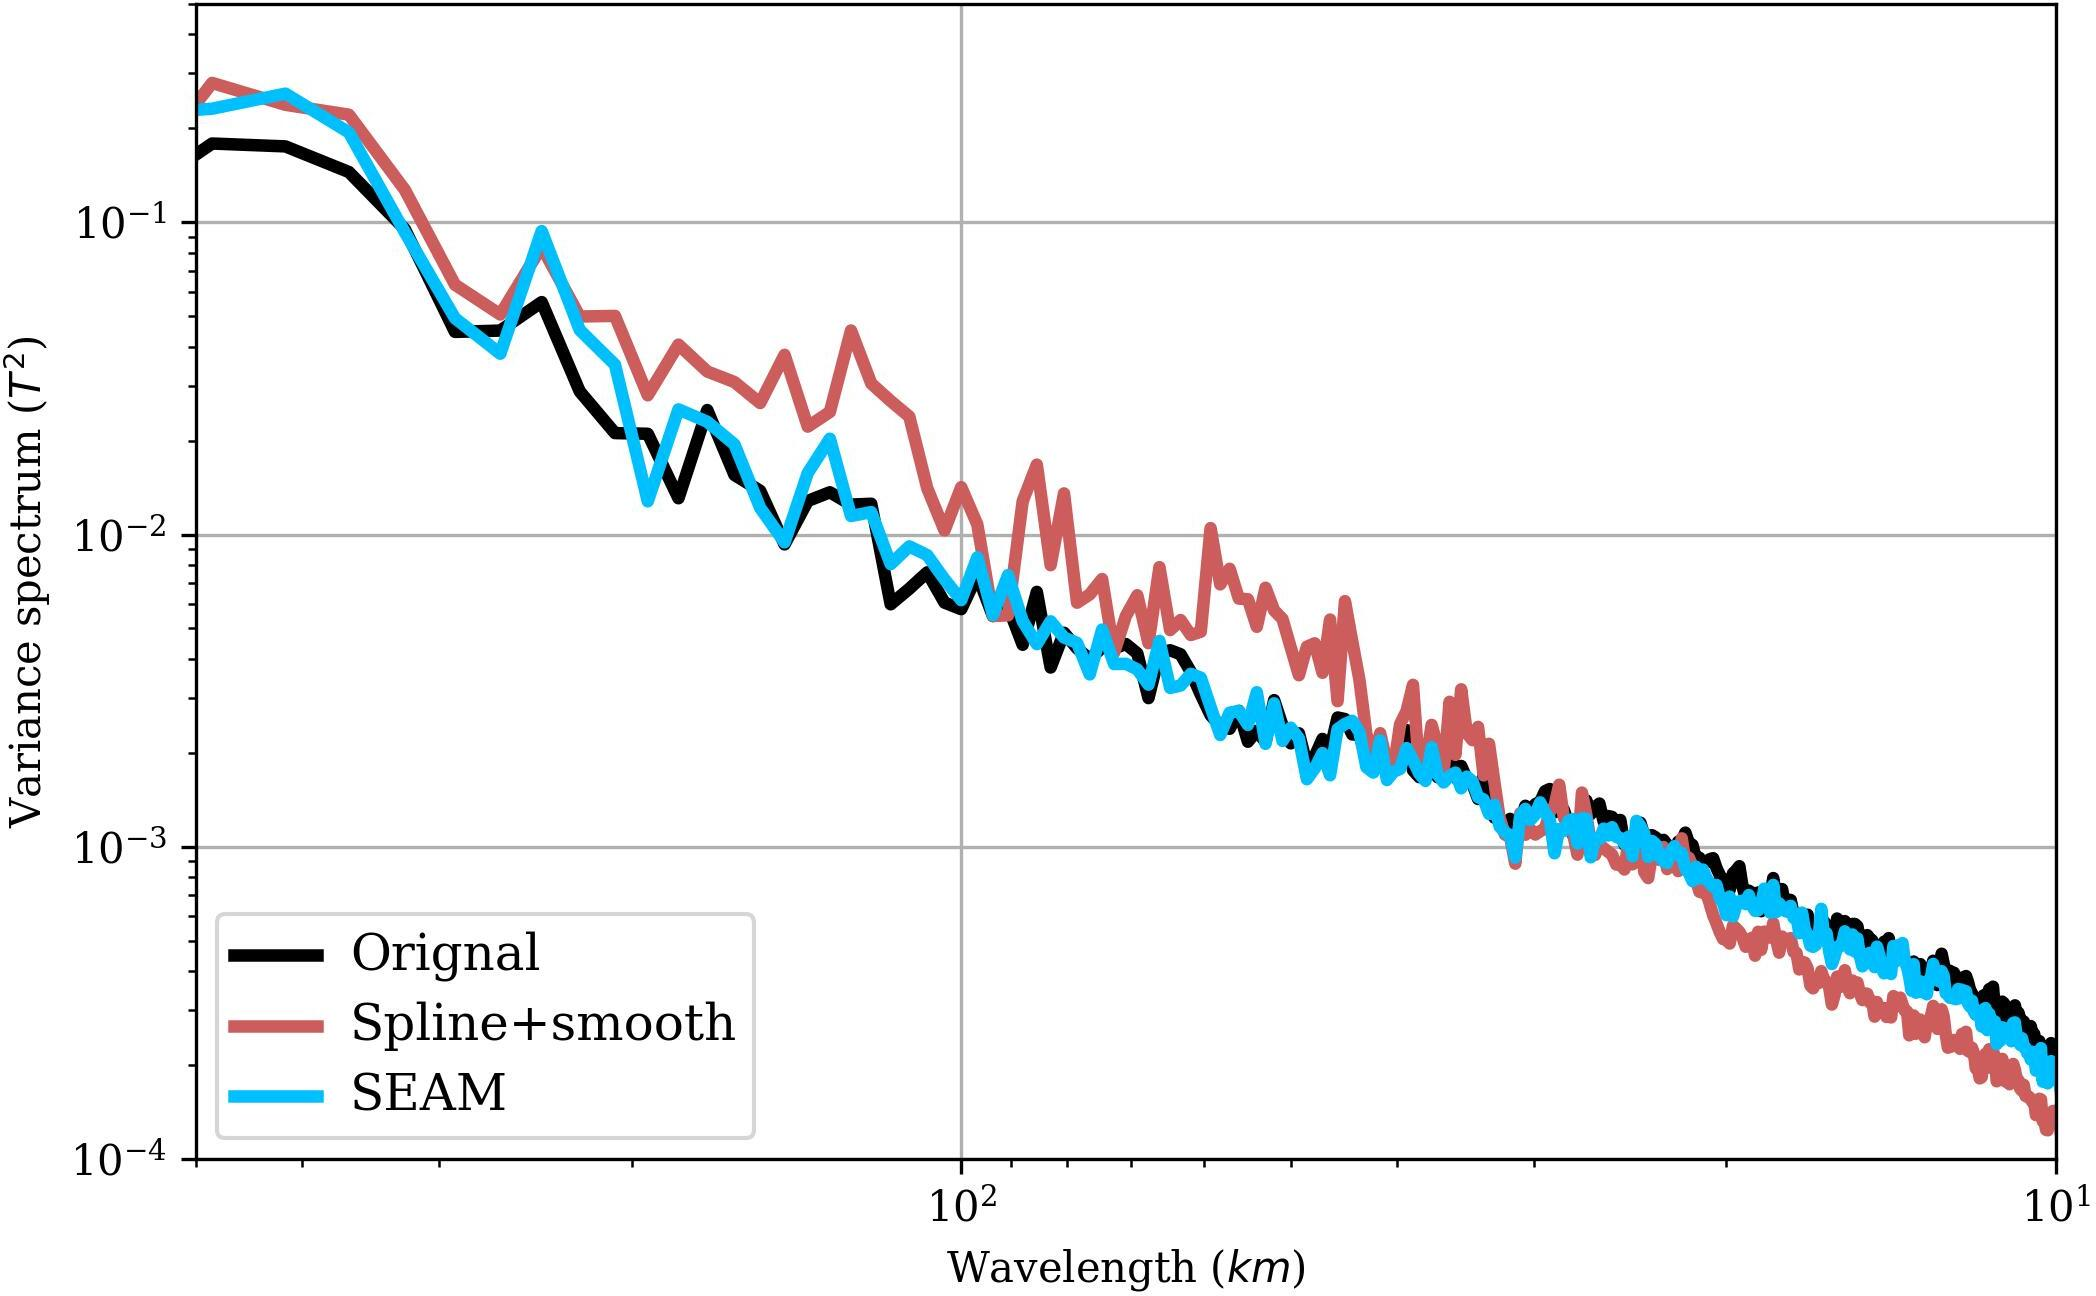
\includegraphics[width=0.7\textwidth]{biperFromIAL_spectra_80_11.jpg}
\caption{Variance spectra of the fields of Figure \ref{fig:biperFromIAL}}
\label{fig:biperFromIAL_spectra_80_11}
\end{figure}
\FloatBarrier

\section{Conclusions}

TBD

\bibliographystyle{mybib-en}
\bibliography{biperiodization}
\end{document}
